% Shared print styling; prose and results live in the Markdown source.
\usepackage{amsmath}
\usepackage{microtype}
\usepackage{float}
\usepackage{needspace}
\usepackage{fancyhdr}
\usepackage{etoolbox}
\usepackage{caption}
\definecolor{labblue}{HTML}{0072B2}
\definecolor{laborange}{HTML}{D55E00}
\definecolor{codebg}{HTML}{F4F6F8}
\AtBeginDocument{\hypersetup{linkcolor=labblue,urlcolor=labblue,citecolor=labblue,pageanchor=false}}
\lstset{
  basicstyle=\fontsize{9}{10.5}\selectfont\ttfamily,
  keywordstyle=\color{labblue}\bfseries,
  commentstyle=\color{black!55},
  stringstyle=\color{laborange},
  backgroundcolor=\color{codebg},
  frame=single,rulecolor=\color{black!12},
  breaklines=true,breakatwhitespace=false,
  columns=fullflexible,keepspaces=true,
  showstringspaces=false,tabsize=4,
  xleftmargin=5pt,xrightmargin=5pt,
  aboveskip=10pt,belowskip=10pt
}
\captionsetup{font=small,labelfont=bf}
\floatplacement{figure}{htbp}
\renewcommand{\topfraction}{0.9}
\renewcommand{\bottomfraction}{0.8}
\renewcommand{\textfraction}{0.1}
\renewcommand{\floatpagefraction}{0.75}
\pagestyle{fancy}
\fancyhf{}
\fancyhead[L]{\small\textcolor{labblue}{LABFIT / PRACTICAL TUTORIAL}}
\fancyhead[R]{\small Synthetic laboratory data}
\fancyfoot[C]{\small\thepage}
\setlength{\headheight}{15pt}
\setlength{\emergencystretch}{3em}
\setlength{\parskip}{4pt}
\raggedbottom
\let\labtoc\tableofcontents
\renewcommand{\tableofcontents}{\begingroup\small\labtoc\endgroup}
\makeatletter
\renewcommand{\maketitle}{
  \begin{titlepage}
  \thispagestyle{empty}
  \vspace*{8mm}
  {\Large\bfseries\color{labblue} LABFIT\par}
  \vspace{5mm}
  {\large A practical laboratory tutorial\par}
  \vspace{10mm}
  {\fontsize{28}{32}\selectfont\bfseries\raggedright\hyphenpenalty=10000\@title\par}
  \vspace{8mm}
  {\Large Fitting, uncertainty and diagnostics\par}
  \vspace{10mm}
  \begin{center}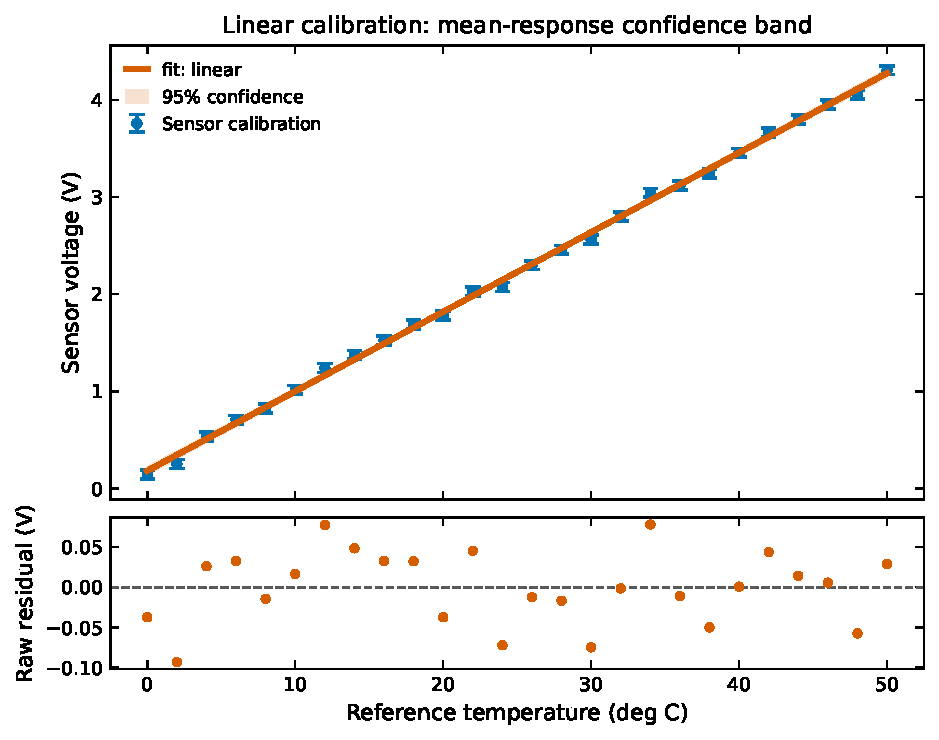
\includegraphics[width=0.95\textwidth,height=80mm,keepaspectratio]{figures/01_calibration.pdf}\end{center}
  \vfill
  {\large Six experiments. One reproducible workflow.\par}
  \vspace{4mm}
  {\normalsize For undergraduate scientists with basic Python knowledge.\par}
  {\normalsize All measurements are synthetic and supplied with the tutorial.\par}
  \vspace{8mm}
  {\small LabFit 0.2.0 \hfill October 2026\par}
  \end{titlepage}
\hypersetup{pageanchor=true}
}
\makeatother
